%----------------------------------------------------------------------------------------
%    PACKAGES AND THEMES
%----------------------------------------------------------------------------------------

\documentclass[aspectratio=169,xcolor=dvipsnames]{beamer}
\usetheme{SimpleDarkBlue}

\usepackage{hyperref}
\usepackage{graphicx} % Allows including images
\usepackage{booktabs} % Allows the use of \toprule, \midrule and \bottomrule in tables

%----------------------------------------------------------------------------------------
%    TITLE PAGE
%----------------------------------------------------------------------------------------

\title{Monthly Research Progress}
\subtitle{April 2025}

\author{Nithish Kumar V}

\institute
{
	Department of Computer Science and Engineering \\
	Indian Institute of Information Technology, Design and Manufacturing, Kancheepuram
}
\date{\today} 

%----------------------------------------------------------------------------------------
%    PRESENTATION SLIDES
%----------------------------------------------------------------------------------------

\begin{document}
	
	\begin{frame}
		% Print the title page as the first slide
		\titlepage
	\end{frame}
	
	\begin{frame}{Overview}
		% Throughout your presentation, if you choose to use \section{} and \subsection{} commands, these will automatically be printed on this slide as an overview of your presentation
		\tableofcontents
	\end{frame}
	\section{Organization of the Survey Paper}
	\begin{frame}{Organization of the Survey Paper}
		\begin{figure}
		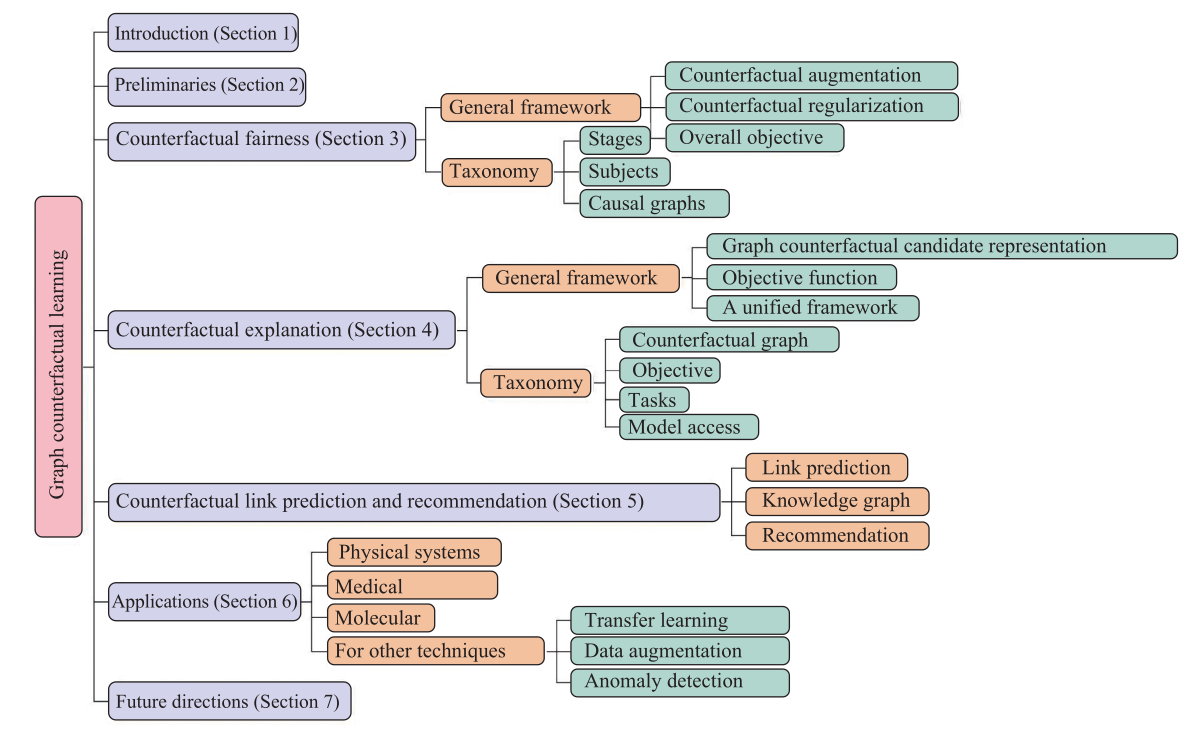
\includegraphics[width=0.8\linewidth]{paper_structure.png}
		\end{figure}
	\end{frame}
	%------------------------------------------------
	\section{Counterfactual Fairness}
	%------------------------------------------------
	
	\begin{frame}{Sources of Bias}
		\begin{itemize}
		\item	The biases in the data lead to unfair predictions
		\item Various sources of bias in any i.i.d (independent and identically distributed data)
			\begin{enumerate}
				\item Historical Bias
				\item Representation Bias
				\item Temporal Bias
				\item Attribute Bias				
			\end{enumerate}
			\item Source of Bias specific to graph data
			\begin{enumerate}
				\item Linking Bias
				\item Structural Bias
			\end{enumerate}
		\end{itemize}
		
	\end{frame}
	
	%------------------------------------------------
	
	\begin{frame}{Counterfactual Fairness}
		
		\begin{itemize}
			\item Biases are measured from different perspectives. 
			\begin{enumerate}
				\item Group fairness 
				\item Individual fairness
			\end{enumerate}
			\item The above metrics rely on the statistical correlation among variables, which may not describe the intrinsic causal structure
			\item Inspired by the development of counterfactual learning, counterfactual fairness is proposed as a notion to measure fairness from the perspective of causal inference
		\end{itemize}
		\begin{block}{Definition}
			Counterfactual fairness makes the outputs of a machine learning model for an individual in the actual world remain the same when we flip the sensitive attribute of the same individual to the counterfactual world.
		\end{block}
		
		

	\end{frame}
	
	%------------------------------------------------
	
	\begin{frame}{General Framework for CF Fairness}
		\begin{columns}[c] % The "c" option specifies centered vertical alignment while the "t" option is used for top vertical alignment
			
			\column{.45\textwidth} % Left column and width
			\textbf{Steps involved}
			\begin{enumerate}
				\item Counterfactual Augmentation
				\item Minimize Discrepancy (Optimization Problem)
			\end{enumerate}
			
			\column{.45\textwidth} % Right column and width
			Possible Research Problems that can be explored
			\begin{enumerate}
				\item Applying Different kinds of Augmentation Techniques
			\end{enumerate}
			
		\end{columns}
	\end{frame}
	
	%------------------------------------------------
	\section{Counterfactual Explanations}
	%------------------------------------------------
	\begin{frame}{Counterfactual Explanations}
		\textbf{Motivation}
		\begin{itemize}
			\item Transparent and interpretable models are essential to ensure that developers understand model behavior and potential biases, and to gain user trust
			\item In drug discovery, GNN interpretations can aid in discovering effective molecular structures
		\end{itemize}
		\begin{block}{Definition}
			Counterfactual explanation on graphs aims to identify the necessary changes to the input graph that can alter the prediction outcome
		\end{block}
	\end{frame}
	\begin{frame}{General Framework for CF Explanation}
		\begin{columns}[c] % The "c" option specifies centered vertical alignment while the "t" option is used for top vertical alignment
			
			\column{.45\textwidth} % Left column and width
			\textbf{Steps involved}
			\begin{enumerate}
				\item Graph counterfactual candidate representation
				\item Optimization
			\end{enumerate}
			
			\column{.45\textwidth} % Right column and width
			Possible Research Problems that can be explored
			\begin{enumerate}
				\item Coming up with different candidate representation
			\end{enumerate}
			
		\end{columns}
		
		\hfill
		
		As discussed in the previous presentation, this can be linked with Pharmacovigilance domain
	\end{frame}
	\section{CF Link Prediction \& Recommendation}
	\begin{frame}{CF Link Prediction \& Recommendation}
		\textbf{Motivation}
		\begin{itemize}
			\item Previous 2 methods are closely related to graph classification tasks
			\item Recommender systems, as a special case of link prediction task, can also benefit from removing spurious information and relying on causal information
		\end{itemize}
		\begin{block}{Definition}
			Counterfactual Link prediction aims to explore the root causes of the formation of links, filtering out the spurious factors
		\end{block}
	\end{frame}
	
	%------------------------------------------------
	
	\begin{frame}{Theorem}
		\begin{theorem}[Mass--energy equivalence]
			$E = mc^2$
		\end{theorem}
	\end{frame}
	
	%------------------------------------------------
	
	\begin{frame}{Figure}
		Uncomment the code on this slide to include your own image from the same directory as the template .TeX file.
		%\begin{figure}
		%\includegraphics[width=0.8\linewidth]{test}
		%\end{figure}
	\end{frame}
	
	
	

	\begin{frame}{Counterfactual Learning on Graphs}
		\begin{itemize}
			\item Recent works on graph counterfactual learning have shown great potential to overcome the aforementioned challenges 	on fairness, explanation, etc.
		\end{itemize}
	\end{frame}
	%------------------------------------------------
	
	\begin{frame}[fragile] % Need to use the fragile option when verbatim is used in the slide
		\frametitle{Citation}
		An example of the \verb|\cite| command to cite within the presentation:\\~
		
		This statement requires citation \cite{p1}.
	\end{frame}
	
	%------------------------------------------------
	
	\begin{frame}{References}
		\footnotesize
		\bibliography{reference.bib}
		\bibliographystyle{apalike}
	\end{frame}
	
	%------------------------------------------------
	
	
	\begin{frame}
		\Huge{\centerline{\textbf{The End}}}
	\end{frame}
	
	%----------------------------------------------------------------------------------------
	
\end{document}
